\begin{enumerate}[label=\thesection.\arabic*.,ref=\thesection.\theenumi]
\numberwithin{equation}{enumi}

\item
What are Constant M and N circles and how can we determine closed loop frequency response using M and N circles?
\solution 
M circles are called constant magnitude Loci and N circles are called as
constant phase angle Loci.These are helpful in determining the closed-loop frequency response of unity negative feedback systems. \\

\textbf{Constant-Magnitude Loci(Mcircle):} Let $G(\j\omega)$ be complex quantity it can be written as 
\begin{align}
G\brak{\j \omega} &= X+\j Y
\end{align}
where X,Y are real quantities.
Let M be magnitude of closed loop transfer function.
\begin{align}
M &= \abs{\frac{X+\j Y}{1+X+\j Y}}
\\
M^{2} &= \frac{X^{2}+Y^{2}}{\brak{1+X}^{2}+Y^{2}}
\label{eq:ee18btech11017_3}
\end{align}

Hence,
\begin{align}
X^{2}\brak{1-M^{2}}-2M^{2}X-M^{2}+\brak{1-M^{2}}Y^{2} &= 0
\label{eq:ee18btech11017_1}
\end{align}

If $M=1$, then from Equation \eqref{eq:ee18btech11017_1}, we obtain $X =\frac{-1}{2}$ This is the equation of a straight line parallel to the Y axis and passing through the point $\brak{\frac{-1}{2},0}$.

If $M \neq 1$ Equation \eqref{eq:ee18btech11017_1} can be written as
\begin{align}
X^{2}+\frac{2M^{2}}{M^{2}-1}X+\frac{M^{2}}{M^{2}-1}+Y^{2} &= 0
\end{align}

Simplifying,
\begin{align}
\brak{X+\frac{M^{2}}{M^{2}-1}}^{2}+Y^{2} &= \frac{M^{2}}{\brak{M^{2}-1}^{2}}
\label{eq:ee18btech11017_2}
\end{align}

Equation \eqref{eq:ee18btech11017_2} is the equation of a circle with center 
$\brak{-\frac{M^{2}}{M^{2}-1},0}$ and radius $\abs{\frac{M}{M^{2}-1}}$

Thus the intersection of Nquist plot with M circle at a frequency($\omega$) results as the magnitude of closed loop transfer function as M at frequency ($\omega$)

\textbf{Constant-Phase-Angle Loci (N Circles):}
Finding Phase angle $\alpha$ from \eqref{eq:ee18btech11017_3} we get,

\begin{align}
\alpha &= \tan^{-1}\brak{\frac{Y}{X}}-\tan^{-1}\brak{\frac{Y}{1+X}}
\\
\text{Let } tan\alpha &= N
\\
N &= tan\brak{\tan^{-1}\brak{\frac{Y}{X}}-\tan^{-1}\brak{\frac{Y}{1+X}}}
\end{align}
Simplifying,
\begin{align}
N &= \frac{Y}{X^{2}+X+Y^{2}}
\end{align}

Further Simplifying..
\begin{align}
\brak{X+\frac{1}{2}}^{2}+\brak{Y-\frac{1}{2N}}^{2} &= \frac{1}{4}+\frac{1}{\brak{2N}^{2}}
\label{eq:ee18btech11017_4}
\end{align}

Equation \eqref{eq:ee18btech11017_4} is the equation of a circle with center at $\brak{\frac{-1}{2},\frac{1}{2N}}$ and radius $\sqrt{\frac{1}{4}+\frac{1}{\brak{2N}^{2}}}$


Thus the intersection of Nquist plot with N circle at a frequency($\omega$) results as the phase of closed loop transfer function as $tan^{-1}\brak{N}$ at frequency ($\omega$)


\item
For unity Feedback system given below,obtain closed loop frequency response using constant M and N circles.
\begin{align}
G\brak{s} &=\frac{50\brak{s+3}}{s\brak{s+2}\brak{s+4}}
\end{align}
\solution
The following code plots Fig. \ref{fig:ee18btech11017}
\begin{lstlisting}
codes/ee18btech11017_1.py
\end{lstlisting}


\begin{figure}[!h]
  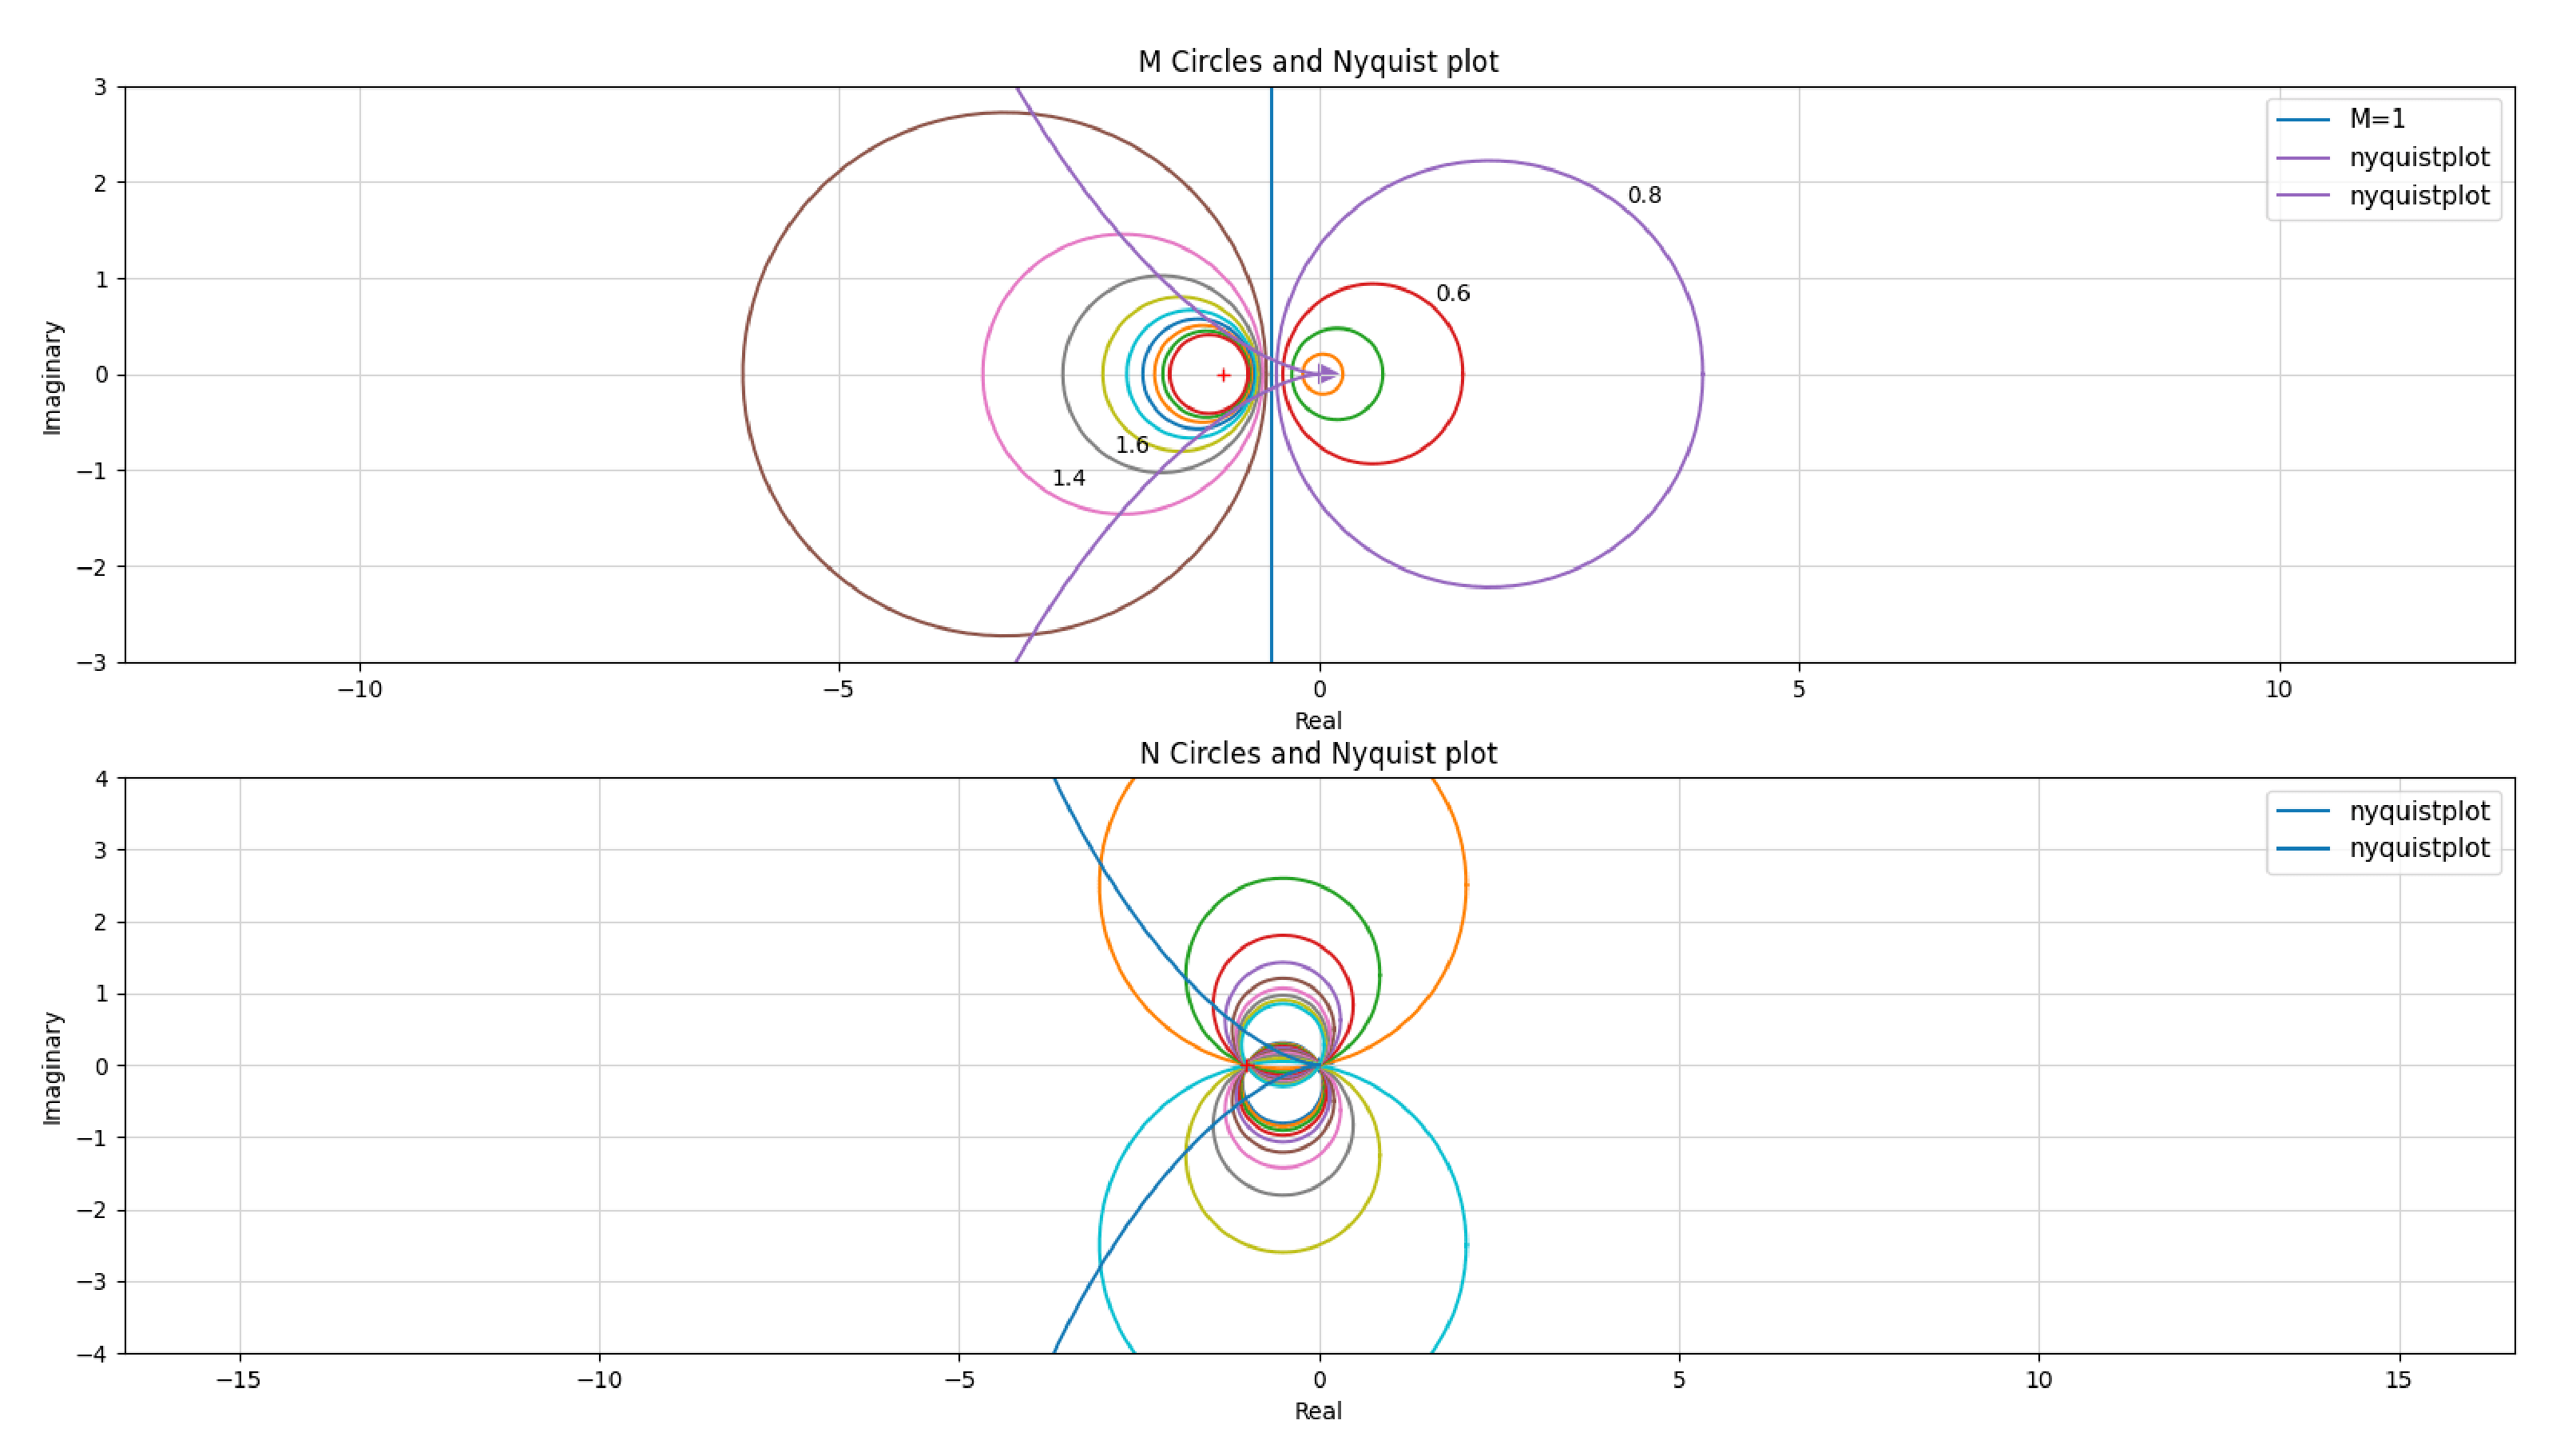
\includegraphics[width=\columnwidth]{./figs/ee18btech11017_fig1.eps}
 \caption{}
  \label{fig:ee18btech11017}
\end{figure}

\item
The following code finds the intersection of M and N circles with Nyquist plot at different frequencies in Table \ref{table:ee18btech11017_table1}
\begin{lstlisting}
codes/ee18btech11017_2.py
\end{lstlisting}


\begin{table}[!ht]
\centering
\input{./tables/ee18btech11017_table1.tex}
\caption{}
\label{table:ee18btech11017_table1}
\end{table}


\item
The following code plots figure(\ref{fig:ee18btech11017_5}), the magnitude plot from the values obtained above in the Table \ref{table:ee18btech11017_table1} along with the original bode plot of the closed loop transfer function.
\begin{lstlisting}
codes/ee18btech11017_3.py
\end{lstlisting}

\begin{figure}[!h]
  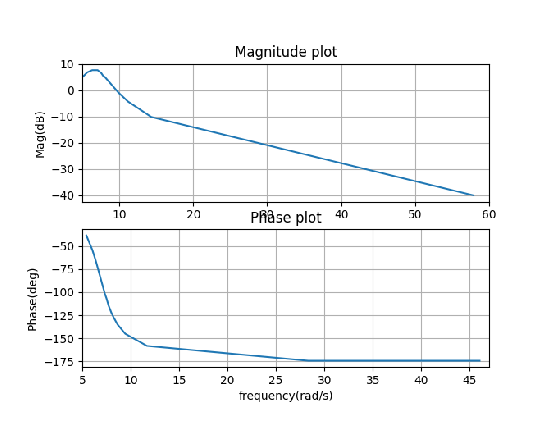
\includegraphics[width=\columnwidth]{./figs/ee18btech11017_fig2.eps}
 \caption{}
  \label{fig:ee18btech11017_5}
\end{figure}






















\end{enumerate}
